% \iffalse
\let\negmedspace\undefined
\let\negthickspace\undefined
\documentclass[journal,12pt,twocolumn]{IEEEtran}
\usepackage{cite}
\usepackage{amsmath,amssymb,amsfonts,amsthm}
\usepackage{algorithmic}
\usepackage{graphicx}
\usepackage{textcomp}
\usepackage{xcolor}
\usepackage{txfonts}
\usepackage{listings}
\usepackage{enumitem}
\usepackage{mathtools}
\usepackage{gensymb}
\usepackage{comment}
\usepackage[breaklinks=true]{hyperref}
\usepackage{tkz-euclide} 
\usepackage{tikz}
\usepackage{circuitikz}
\usepackage{listings}
\usepackage{gvv}                                        
\def\inputGnumericTable{}                                 
\usepackage[latin1]{inputenc}                                
\usepackage{color}                                            
\usepackage{array}                                            
\usepackage{longtable}                                       
\usepackage{calc}                                             
\usepackage{multirow}                                         
\usepackage{hhline}                                           
\usepackage{ifthen}                                           
\usepackage{lscape}
\usepackage{caption}
\newtheorem{theorem}{Theorem}[section]
\newtheorem{problem}{Problem}
\newtheorem{proposition}{Proposition}[section]
\newtheorem{lemma}{Lemma}[section]
\newtheorem{corollary}[theorem]{Corollary}
\newtheorem{example}{Example}[section]
\newtheorem{definition}[problem]{Definition}
\newcommand{\BEQA}{\begin{eqnarray}}
\newcommand{\EEQA}{\end{eqnarray}}
\newcommand{\define}{\stackrel{\triangle}{=}}
\theoremstyle{remark}
\newtheorem{rem}{Remark}
\begin{document}
\parindent 0px
\bibliographystyle{IEEEtran}
\vspace{3cm}

\title{GATE 2022 33.BM}
\author{EE23BTECH11012 - Chavan Dinesh$^{*}$% <-this % stops a space
}
\maketitle
\newpage
\bigskip

\renewcommand{\thefigure}{\arabic{figure}}
\renewcommand{\thetable}{\arabic{table}}
\large\textbf{\textsl{Question:}}
A series RLC circuit with $R = 10 \Omega$, $L = 50 mH$ and $C = 100 \micro F$ connected to
$200$ V, $50$ Hz supply consumes power P. The value of L is changed such that this
circuit consumes same power P but operates with lagging power factor. The new
value of L is $\_\_\_\_\_$ mH (rounded off to two decimal places).
\hfill(GATE 33 BM 2022)

\solution

\begin{table}[htbp]
    \centering
    \begin{tabular}{|c|c|c|}
\hline
   \textbf{Parameter}  & \textbf{Description} & \textbf{Value}\\
   \hline
   R   & Resistance & $10 \omega$\\
   \hline
  C & Capacitance & $100 \micro F$ \\
  \hline
  L & Inductor & $50mH$\\
  \hline
  Z & Impedance & \\
  \hline
  $Z_{new}$ &New Impedance & \\
  \hline
\end{tabular}

    \caption{}
    \label{tab:input_parameters.33.BM.2022}
\end{table}

\begin{figure}[!ht]
    \centering
        \begin{circuitikz}
    \draw(0, 0) -- (1, 0);
    \draw(1, 0) to [L, l = $50\text{mH}$](2, 0);
    \draw(2, 0) -- (3, 0);
    \draw(3, 0) to [C, l = $100\, \mu\text{F}$](4, 0);
    \draw(4, 0) -- (5, 0);
    \draw(5, 0) to [R, l = $10\Omega$](6, 0);
    \draw(0, 0) -- (0, -2);
    \draw[->] (0, -1) node[left] {$I(t)$} -- (0, -1);
    \draw(6, 0) -- (7, 0);
    \draw(7, 0) -- (7, -2);
    \draw(0, -2) -- (3, -2);
    \draw(7, -2) -- (7, -2);
    \draw(3, -2) to [sV, l = $V(t)$](4, -2);
    \draw(4, -2) -- (7, -2);
\end{circuitikz}

    \caption{}
    \label{fig:fig1.33.BM.2022}
\end{figure}

From \figref{fig:fig1.33.BM.2022}

In s - domain,
\begin{figure}[htbp]
    \centering
    \begin{circuitikz}
    \draw(0, 0) -- (1, 0);
    \draw(1, 0) to [L, l = $sL$](2, 0);
    \draw(2, 0) -- (3, 0);
    \draw(3, 0) to [C, l = $\frac{1}{sC}$](4, 0);
    \draw(4, 0) -- (5, 0);
    \draw(5, 0) to [R, l = $R$](6, 0);
    \draw(0, 0) -- (0, -2);
    \draw[->] (0, -1) node[left] {$I(s)$} -- (0, -1);
    \draw(6, 0) -- (7, 0);
    \draw(7, 0) -- (7, -2);
    \draw(0, -2) -- (3, -2);
    \draw(7, -2) -- (7, -2);
    \draw(3, -2) to [sV, l = $V(s)$](4, -2);
    \draw(4, -2) -- (7, -2);
\end{circuitikz}

\end{figure}

 \begin{align}
         Z &= R +j(X_l - X_c)\\ 
         Z &= R +j\left(2\pi fL - \frac{1}{2\pi fC}\right)\label{eq:Z_impedence.bm.33.2022}
 \end{align}
From \tabref{tab:input_parameters.33.BM.2022}:
  \begin{align}
      Z = 10 -  16.123 j 
  \end{align}
As the circuit consumes same power P but operates with lagging power factor : 

The new impedance($Z_{new}$) will be :
\begin{align}
    Z_{new}=  10 + 16.123 j =  R +j\left(2\pi fL_{new} - \frac{1}{2\pi fC}\right)
\end{align}
Comparing the imaginary parts of the $Z_{new}$:

\begin{align}
    L_{new} \approx 152.7 \text{mH}
\end{align}

% \begin{figure}[ht]
%     \centering
%     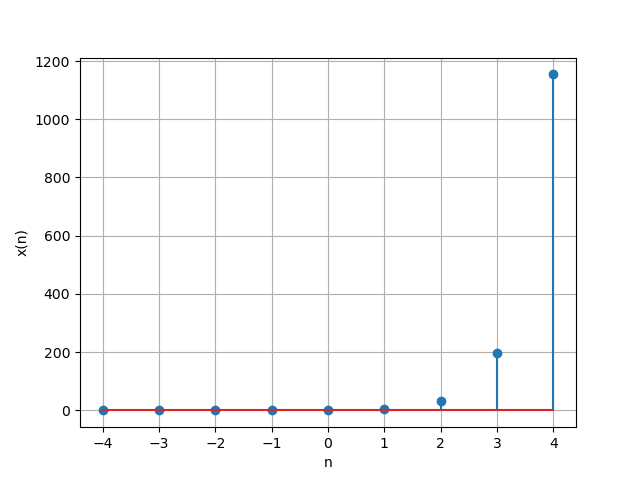
\includegraphics[width = \columnwidth]{figs/x_n_stem_plot.png}
%     \caption{}
%     \label{fig:graph1.11.9.3.28}
% \end{figure}

\bibliographystyle{IEEEtran}
\end{document}
